\newcommand{\as}{\glqq}
\newcommand{\ad}{\grqq}
\newcommand{\adl}{\grqq{ }}

\newcommand{\fref}[1]{Abb. \ref{#1}} %Ref Figures

\section{Einleitung}
    Im Rahmen dieser Ausarbeitung werde ich die AMCON Software GmbH (AMCON) vorstellen und herausarbeiten, welche 
    Aufbauorganisationen und Führungskonzepte in diesem Unternehmen angewandt werden.

    Als erstes möchte ich AMCON einmal vorstellen. Dabei gehe ich auf die historische Entstehung und die Entwicklung des 
    Unternehmens bis heute ein. Ich werde auf die verschiedenen Aufbauorganisationen und Führungskonzepte eingehen und 
    zeigen wie diese bei AMCON Anwendung finden. Des weiteren wird anhand des Entwicklungsteams, in welchem ich arbeite 
    die unterste Führungsebene vorgestellt wobei ich auf die Vor-und Nachteile der Teamstruktur bei AMCON eingehen 
    möchte. Zum Schluss möchte ich einen kurzen Rückblick auf das Projekt geben.


\section{AMCON Software GmbH}
    Das IT-Unternehmen AMCON hat seinen Sitz in der Stadt Cloppenburg und entwickelt hauptsächlich Software für die 
    Branche des öffentliche Personennahverkehrs (ÖPNV). In den folgenden beiden Abschnitten werde ich einmal das 
    Unternehmen AMCON und dessen Leitbild vorstellen und danach auf die näher auf die Historische Entwicklung von AMCON 
    eingehen. In diesen Abschnitten werden Informationen aus der Internen Dokumentation von AMCON verwendet. Diese 
    werden nicht weiter im Quellenverzeichnis aufgeführt.

    \subsection{Unternehmensprofil}
        Das IT-Unternehmen AMCON mit Sitz in Cloppenburg ist über den Zeitraum der letzten 12 Jahre sehr stark 
        gewachsen. Wo das Unternehmen im Jahr 2010 nur 3 Mitarbeiter hatte, sind es jetzt circa 100 Menschen welche hier
        jeden Tag arbeiten. Auch hat AMCON mittlerweile einen Kundenstamm von über 50 Kunden aus dem Bereich des ÖPNV
        aufgebaut. (Vgl. \cite{AMC22c})

        Zu den Produkten von AMCON gehört einmal die zentrale Verwaltungssoftware, das Hintergrundsystem, welches im 
        späteren Verlauf noch näher beschrieben wird. Auch bietet AMCON Softwarelösungen für Ticketautomaten und  
        Verkaufssysteme in öffentlichen Verkehrsmitteln. Ein weiteres Produkt von AMCON wären die Lösungen für Webshops,
        mit welchen die Kunden der ÖPNV-Unternehmen Online Tickets kaufen und Bestellungen verwalten können.

        Das Leitbild des Unternehmens setzt sich zusammen aus der Zufriedenheit der Kunden und der Mitarbeiter, welche
        bei AMCON eine hohe Priorität haben, aber auch die Qualität der Produkte hat bei AMCON einen hohen Stellenwert 
        weshalb seit diesem Jahr ein dediziertes Team aus Testern gibt, welche sich darum kümmern, das Fehler gefunden 
        werden bevor die beim Kunden landen. Um die Bindung zu den Mitarbeitern und Kunden zu stärken, gibt es 
        regelmäßig Events wie zum Beispiel das Sommerfest oder unsere monatlichen Mitarbeiterrunden. Für die Kunden 
        veranstaltet AMCON jährlich eine Boßeltour. (Vgl. \cite{AMC22c})

        Da AMCON als IT-Unternehmen auch vom Fachkräftemangel betroffen ist, hat AMCON es sich zur Aufgabe gemacht, hier
        entgegen zu wirken. Allein über 20 der aktuell etwa 100 Mitarbeitern sind Auszubildende und Duale Studenten.
        Auch engagiert AMCON sich an Schulen und arbeitet mit diesen zusammen, um junge Menschen für die IT zu 
        begeistern. Hierfür nimmt das Unternehmen auch am alljährlichen Zukunftstag teil, bei welchem Kinder von der 
        5. bis zur 10. Klasse einen Einblick in den Alltag eines Softwareentwicklers bekommen. Durch dieses Engagement 
        in Schulen und auf Jobmessen hat AMCON auch ein sehr junges Team aufgebaut, welches einen Altersdurchschnitt von
        nur 30 Jahren hat. (Vgl. \cite{AMC22c})
        \pagebreak

    \subsection{Historische Entwicklung von AMCON}
        AMCON ist ein Unternehmen welches 1992 als der Universitätsprojekt begonnen hat. Prof. Dr. Dr. h.c. Sönke Albers
        und Bernd Michalk haben das Unternehmen damals noch bekannt unter dem Namen AMCON Analytical Marketing 
        Consulting GmbH an der Universität in Kiel gegründet. Olaf Clausen, welcher Student an der Universität war,
        arbeitete hier als Studentischer Mitarbeiter.

        Durch ein Projekt der S-Bahn Hamburg  hatte AMCON im Jahr 1994 den erste Kontakt mit der Softwareentwicklung
        und setzte die erste Softwarelösung für die Branche des ÖPNV um. Hierbei handelte es sich um eine Software, mit
        welcher die S-Bahn Hamburg Job-Tickets verwalten konnte.

        Im Jahr 1999 wurde der Sitz der Firma von Kiel in die Stadt Cloppenburg verlegt, wo das Unternehmen auch bis 
        heute ansässig ist. Im selben Jahr trat Olaf Clausen auch in die Geschäftsführung ein. Darius Rauert, welcher 
        heute zusammen mit Olaf Clausen die Geschäftsführung übernimmt, hat zu dieser Zeit als Aushilfe bei AMCON 
        gearbeitet.

        Noch vor 12 Jahren hatte AMCON nur drei Mitarbeiter und war damit ein sehr kleines Unternehmen. 2010 war Olaf
        Clausen alleiniger Gesellschafter während Darius Rauert als Prokurist in die Geschäftsführung mit eingestiegen
        ist. 4 Jahre später wurde die Führung des Unternehmens zwischen Olaf und Darius aufgeteilt, als Darius im Jahr
        2014 50\% der Firmenanteile übernahm.

        Noch im selben Jahr erhielt AMCON den Zuschlag für ein Projekt bei Harzer Schmalspurbahn, womit AMCON erstmals
        mehr Aufmerksamkeit in der ÖPNV - Branche bekam.

        Um weiter zu wachsen und eine größere Aufmerksamkeit zu bekommen, hat ist AMCON seit dem Jahr 2016 auch auf 
        Job- und Fachmessen vertreten. Außerdem wurde AMCON in diesem Jahr auch nach dem ISO 9001:2015 Standard 
        zertifiziert. Des weiteren war AMCON auch auf der größten Jobmesse für die Branche des ÖPNV, der InnoTrans in 
        Berlin vertreten.

        In den Jahren 2018 bis 2020 gab es eigne Änderungen in der generellen Struktur und Aufbauorganisation. Es wurden
        die neuen Führungsebenen der Teamleiter und der Produktverantwortlichen eingeführt. Dazu wurde im Jahr 2020 auf
        das Projektmanagement dahingehend geändert, das nun der SCRUM-Prozess im gesamten Betrieb angewandt wird.

        Heute in 2022 hat AMCON circa 100 Mitarbeiter und arbeitet verteilt auf vier Standorten in Cloppenburg. Die 
        Aufteilung auf mehrere Standorte ist allerdings nicht immer eine gute Lösung weshalb AMCON ein neues 
        Bürogebäude bauen möchte. Diese soll bis zum Jahr 2025 in der Gemeinde Molbergen entstehen, in welchem dann alle
        Mitarbeiter von AMCON platz finden.
        \pagebreak

\section{Organisationsformen} \label{Organisationsformen}
    In diesem Kapitel werden einmal die verschiedenen Formen der Organisation mit ihren Vor- und Nachteilen vorgestellt.
    Im Anschluss wird dann ein Bezug zum Unternehmen AMCON hergestellt, in welchem gezeigt wird, ob und wie diese Formen
    im Unternehmen zum Einsatz kommen.

    \subsection{Einliniensystem} \label{Einliniensystem}
        Im Einliniensystem gibt es eine hierarchische Struktur mit einer klar abgegrenzten Weisungskompetenz. Auf diese 
        Weise bekommt ein Arbeitnehmer aus dem Bereich Materialwirtschaft nur Weisung von Abteilungsleiter der 
        Materialwirtschaft. Dazu gibt es bei Fragen und Problemen immer einen klaren Ansprechpartner. Der Aufbau des 
        Einliniensystems ist auch in \fref{Einlinie} noch einmal grafisch dargestellt.
        (Vgl. \cite{Woehe2020} S.\,111-112)

        Allerdings hat das Einliniensystem auch einen großen Nachteil. Durch die klare Abgrenzung der Abteilungen und 
        Teilbereiche gibt es sehr lange und umständliche Kommunikationswege. Wenn nun ein Arbeitnehmer aus der 
        Abteilungen Materialwirtschaft eine Frage an den Abteilungsleiter Vertrieb hat, muss dieser zuerst seinen 
        Abteilungsleiter ansprechen. Dieser würde dann das Anliegen an die Geschäftsführung weiterleiten. Von dort wird 
        dann der Abteilungsleiter Vertrieb angesprochen. Die Antwort auf die Frage muss nun den selben Weg wieder zurück
        nehmen. Dieses Problem macht das Einliniensystem vor allem im Bereich Kommunikation sehr ineffizient. 
        (Vgl. \cite{Woehe2020} S.\,111-112)

        \begin{figure}[ht]
            \centering
            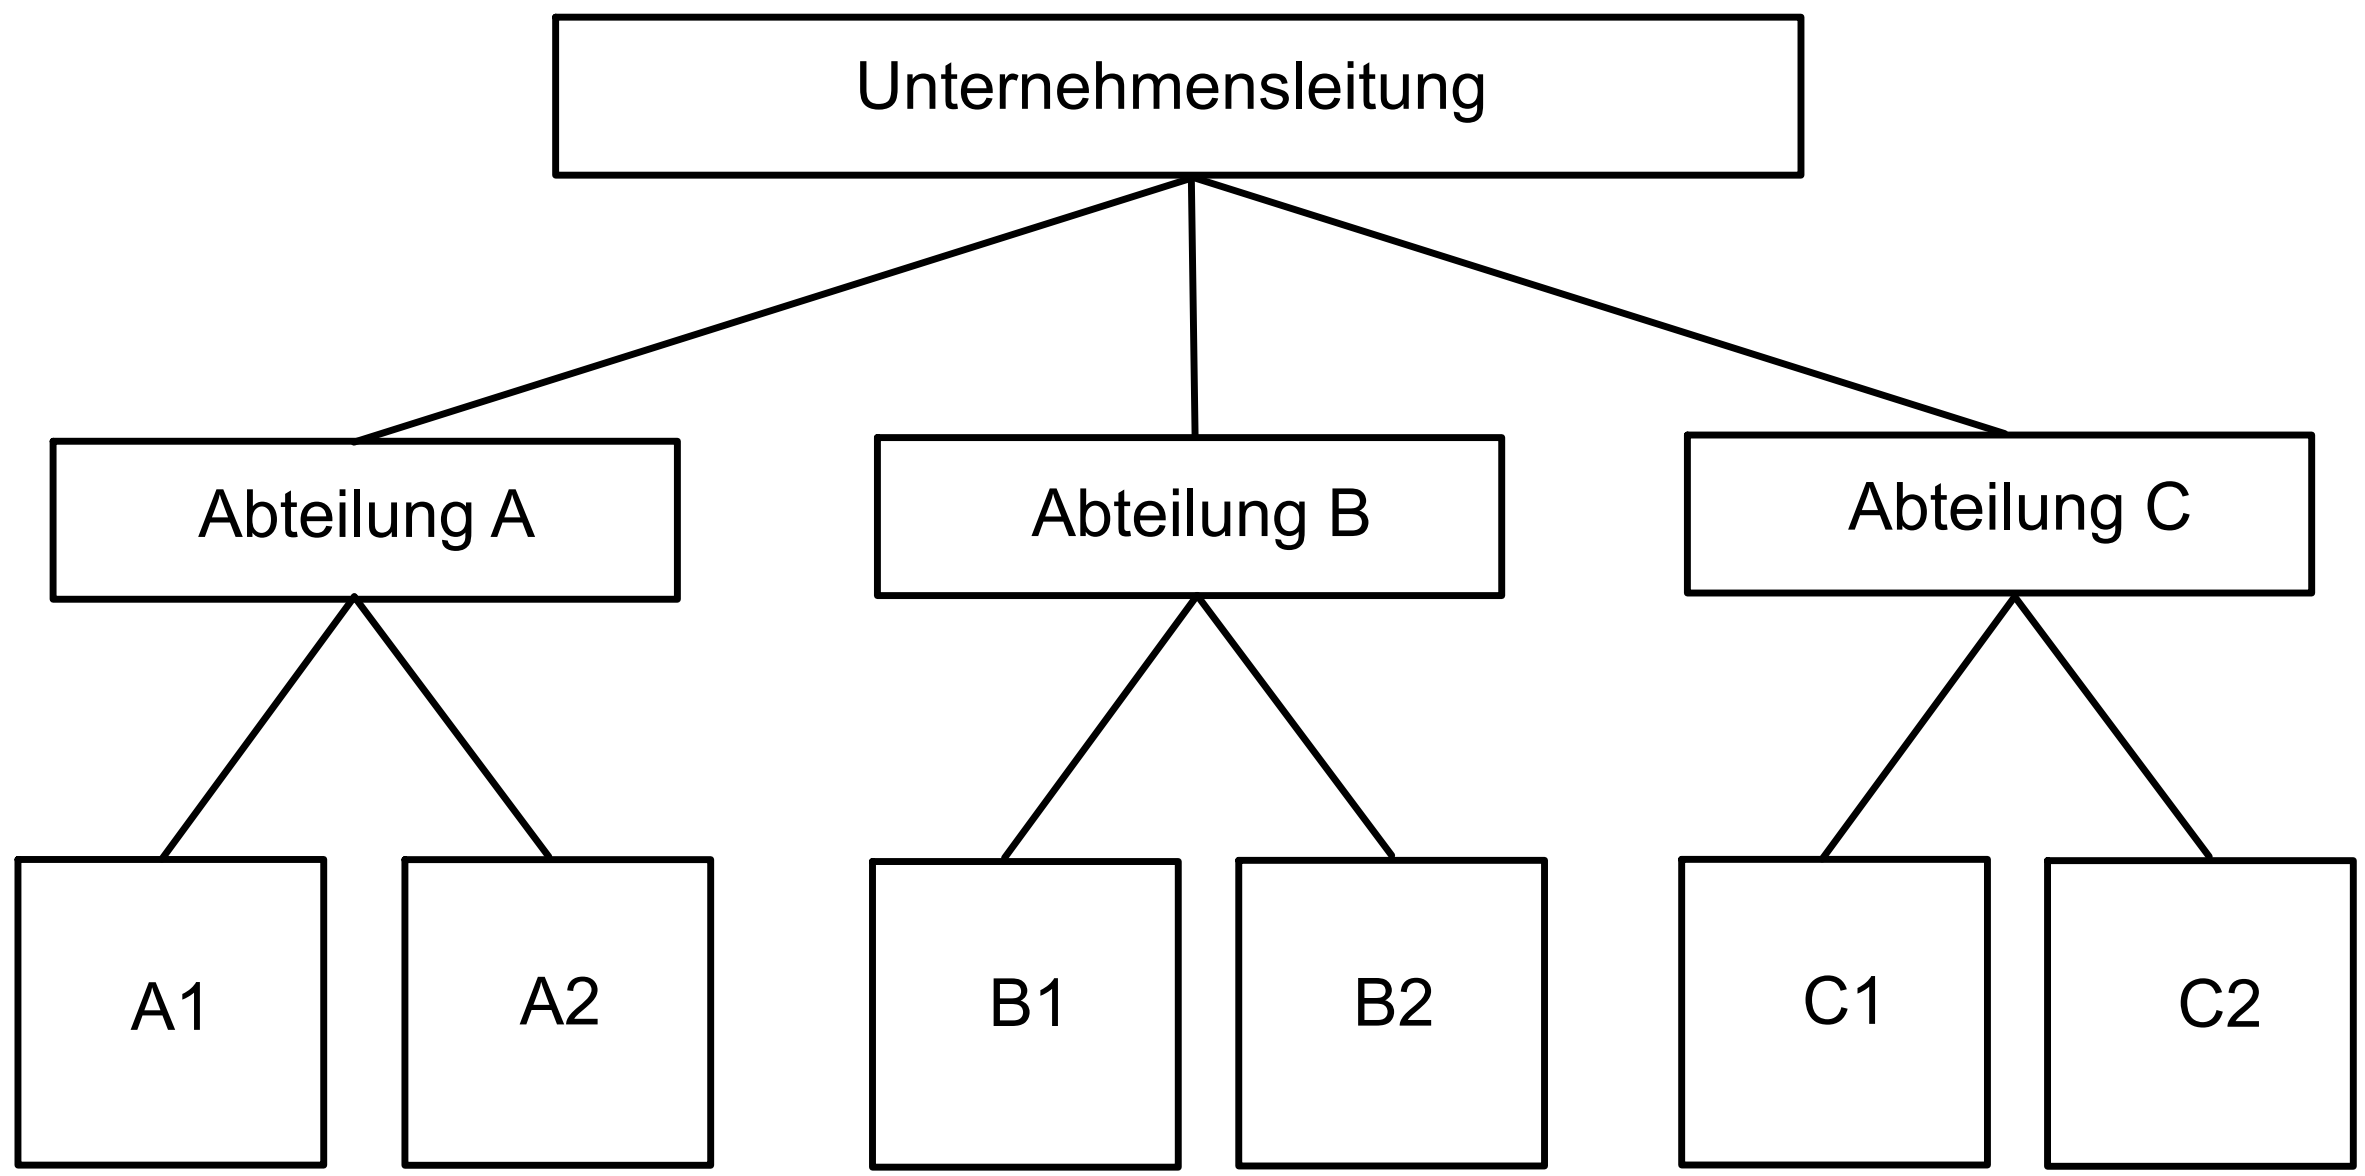
\includegraphics[width = 0.8\textwidth]{Eigene Darstellungen/Einliniensystem.PNG}

            \caption{Einliniensystem (Eigene Darstellung, in Anlehnung an \cite{Woehe2020} S.\,112)} \label{Einlinie}
        \end{figure}
    
    \subsection{Mehrliniensystem} \label{Mehrliniensystem}
        Das Mehrliniensystem ist hat allgemein einen sehr ähnlichen Aufbau zum Einliniensystem, welcher auch in 
        \fref{Mehrlinie} noch einmal grafisch dargestellt wird. Der Unterschied ist, dass die Kommunikationswege 
        vereinfacht und verkürzt werden. Wenn nun wieder ein Arbeitnehmer aus der Abteilungen Materialwirtschaft eine 
        Frage an dan Abteilungsleiter Vertrieb hat, kann dieser einfach die Frage an diese Person stellen und muss nicht
        den Umweg über seinen Abteilungsleiter gehen. Dies vereinfacht die Kommunikation soweit, dass es schneller eine 
        Antwort auf ein Frage gibt und somit viel zeit gespart wird, welche für die Erledigung der eigentlichen Aufgaben
        verwendet werden kann. (Vgl. \cite{Woehe2020} S.\,112)

        Allerdings hat das Mehrliniensystem auch einen Nachteil. Der Arbeitnehmer ist hier der \as Diener Zweier 
        Herren\ad. Das bedeutet, dass der Arbeitnehmer mehr als einen Vorgesetzten hat, was dazu führen kann, das dieser 
        Aufträge bekommt, welche miteinander im Konflikt stehen. Somit muss dann erst geregelt werden, was genau der 
        Arbeitnehmer wirklich machen soll. Außerdem ist bei in diesem System nicht immer klar, wer bei Fragen der 
        Ansprechpartner ist. (Vgl. \cite{Woehe2020} S.\,112)

        \begin{figure}[h]
            \centering
            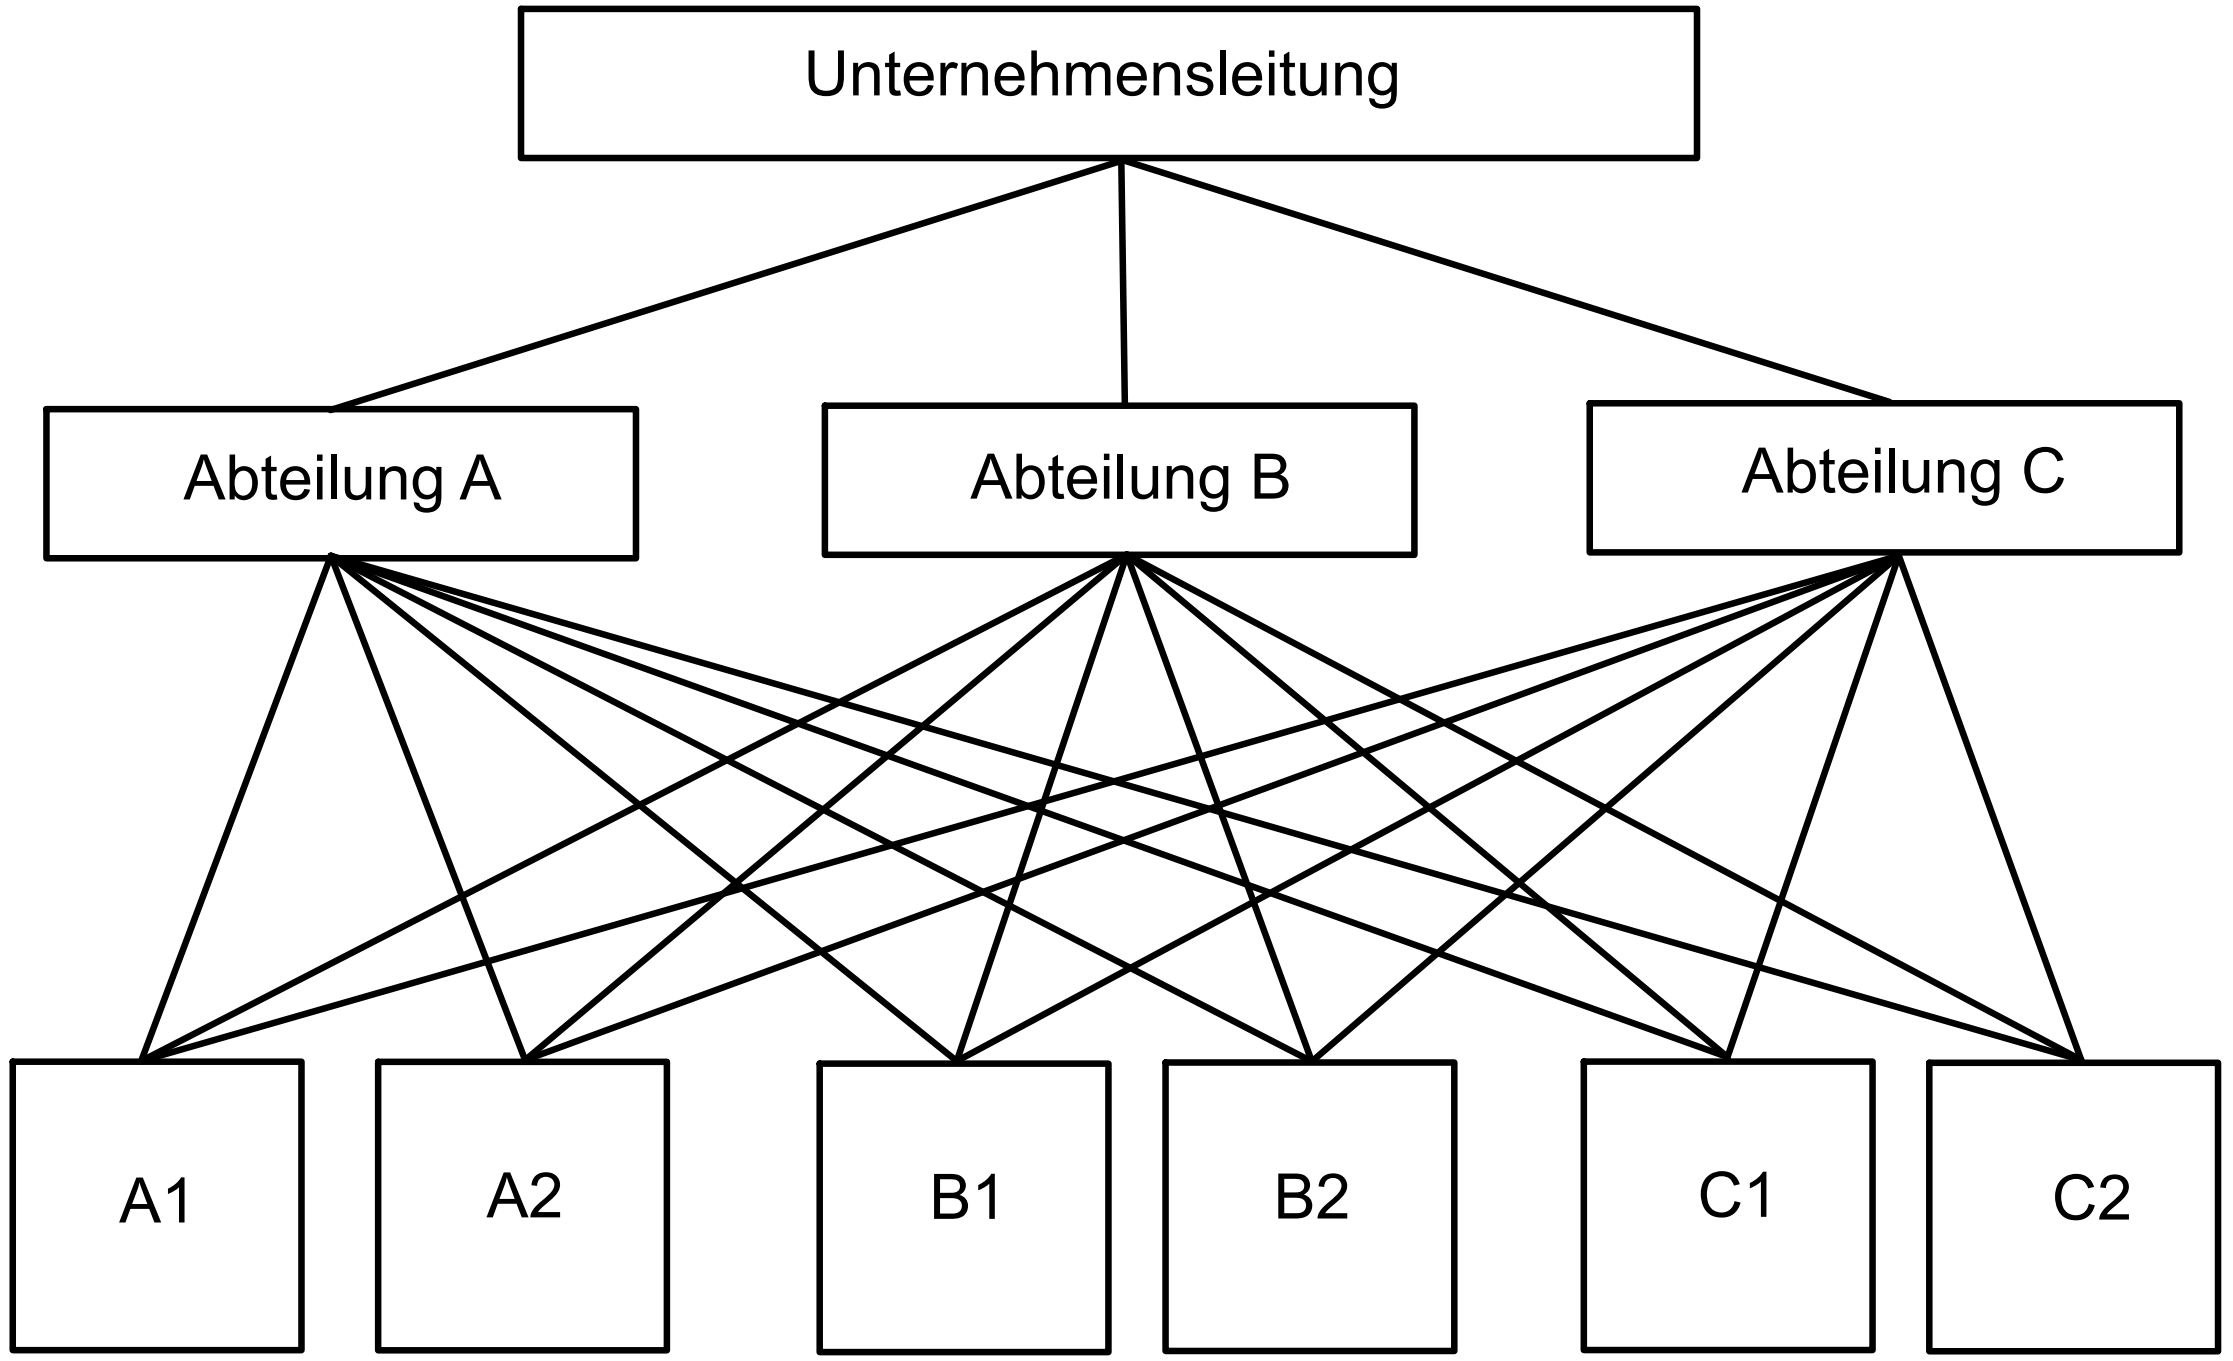
\includegraphics[width = 0.8\textwidth]{Eigene Darstellungen/Mehrliniensystem.PNG}
            \caption{Mehrliniensystem (Eigene Darstellung, in Anlehnung an \cite{Woehe2020} S.\,112)} \label{Mehrlinie}
        \end{figure}

    \subsection{Stabliniensystem}   \label{Stablinienorganisation}
        Bei schnell wachsenden Unternehmen mit einem Ein- oder Mehrliniensystem kann es schnell zu einer sehr komplexen 
        und unübersichtlichen Organisationsstruktur kommen. Durch das Stabliniensystem kann die Organisation vereinfacht
        werden. Dieses System hat eine große Ähnlichkeit zum Einliniensystem (\ref{Einliniensystem}) mit dem Unterschied
        das es an jeder Führungsebene eine sogenannte \as Stabstelle\adl gibt. Diese Stabstellen haben selbst kein 
        Weisungsrecht und nehmen nur Weisung von \as ihrer\adl entgegen. Die Instanz in welche sie sich befinden ist 
        die Abteilung, zu welcher sie gehören. Am besten kann dieses System an einem Beispiel erklärt werden. Das 
        Personalwesen ist eine Zentralstelle an der Unternehmensleitung. Nun nimmt das Personalwesen Weisung von der 
        Unternehmensleitung, und hat ein eingeschränktes Weisungsrecht in Form von Beratung. Das Personalwesen kann in 
        Bereichen wie der Einstellung, Entlassung oder den Mitarbeiterqualifikationen eine beratende Rolle übernehmen.
        Der Aufbau des Stabliniensystems  ist auch in der \fref{Stablinie} noch einmal grafisch dargestellt.
        (Vgl. \cite{Woehe2020} S.\,112-113)

        Dann gibt es noch den Fall das eine Stabstelle an einer Abteilung gibt. Nehmen wir einmal die Abteilungen 
        Marketing. An dieser Abteilung gibt es die Stabstelle \as Marktforschung\ad. Diese Stabstelle hat selbst kein
        Weisungsrecht in der Abteilung, nimmt aber der Leitung Arbeit ab, bzw. nimmt Weisung von der Abteilungsleitung 
        an und kann sich besser über die Themen der Marktforschung beraten, da diese ein höheres Maß an Fachwissen hat.
        (Vgl. \cite{Woehe2020} S.\,112-113)
        
        Aber es gibt keine Lösung welche nur Vorteile hat. So ist es im Stabliniensystem so, dass Entscheidungsprozesse 
        unübersichtlich werden können, da die Entscheidungen zum Beispiel von einer Stabstelle getroffen werden, aber
        die Ausführung dieser Entscheidungen bei der Führungsinstanz liegt. Auch können so Probleme auftreten, wenn es
        verschiedene Stabstellen gibt, die Entscheidungen treffen, welche zueinander im Konflikt stehen.

        \begin{figure}[ht]
            \centering
            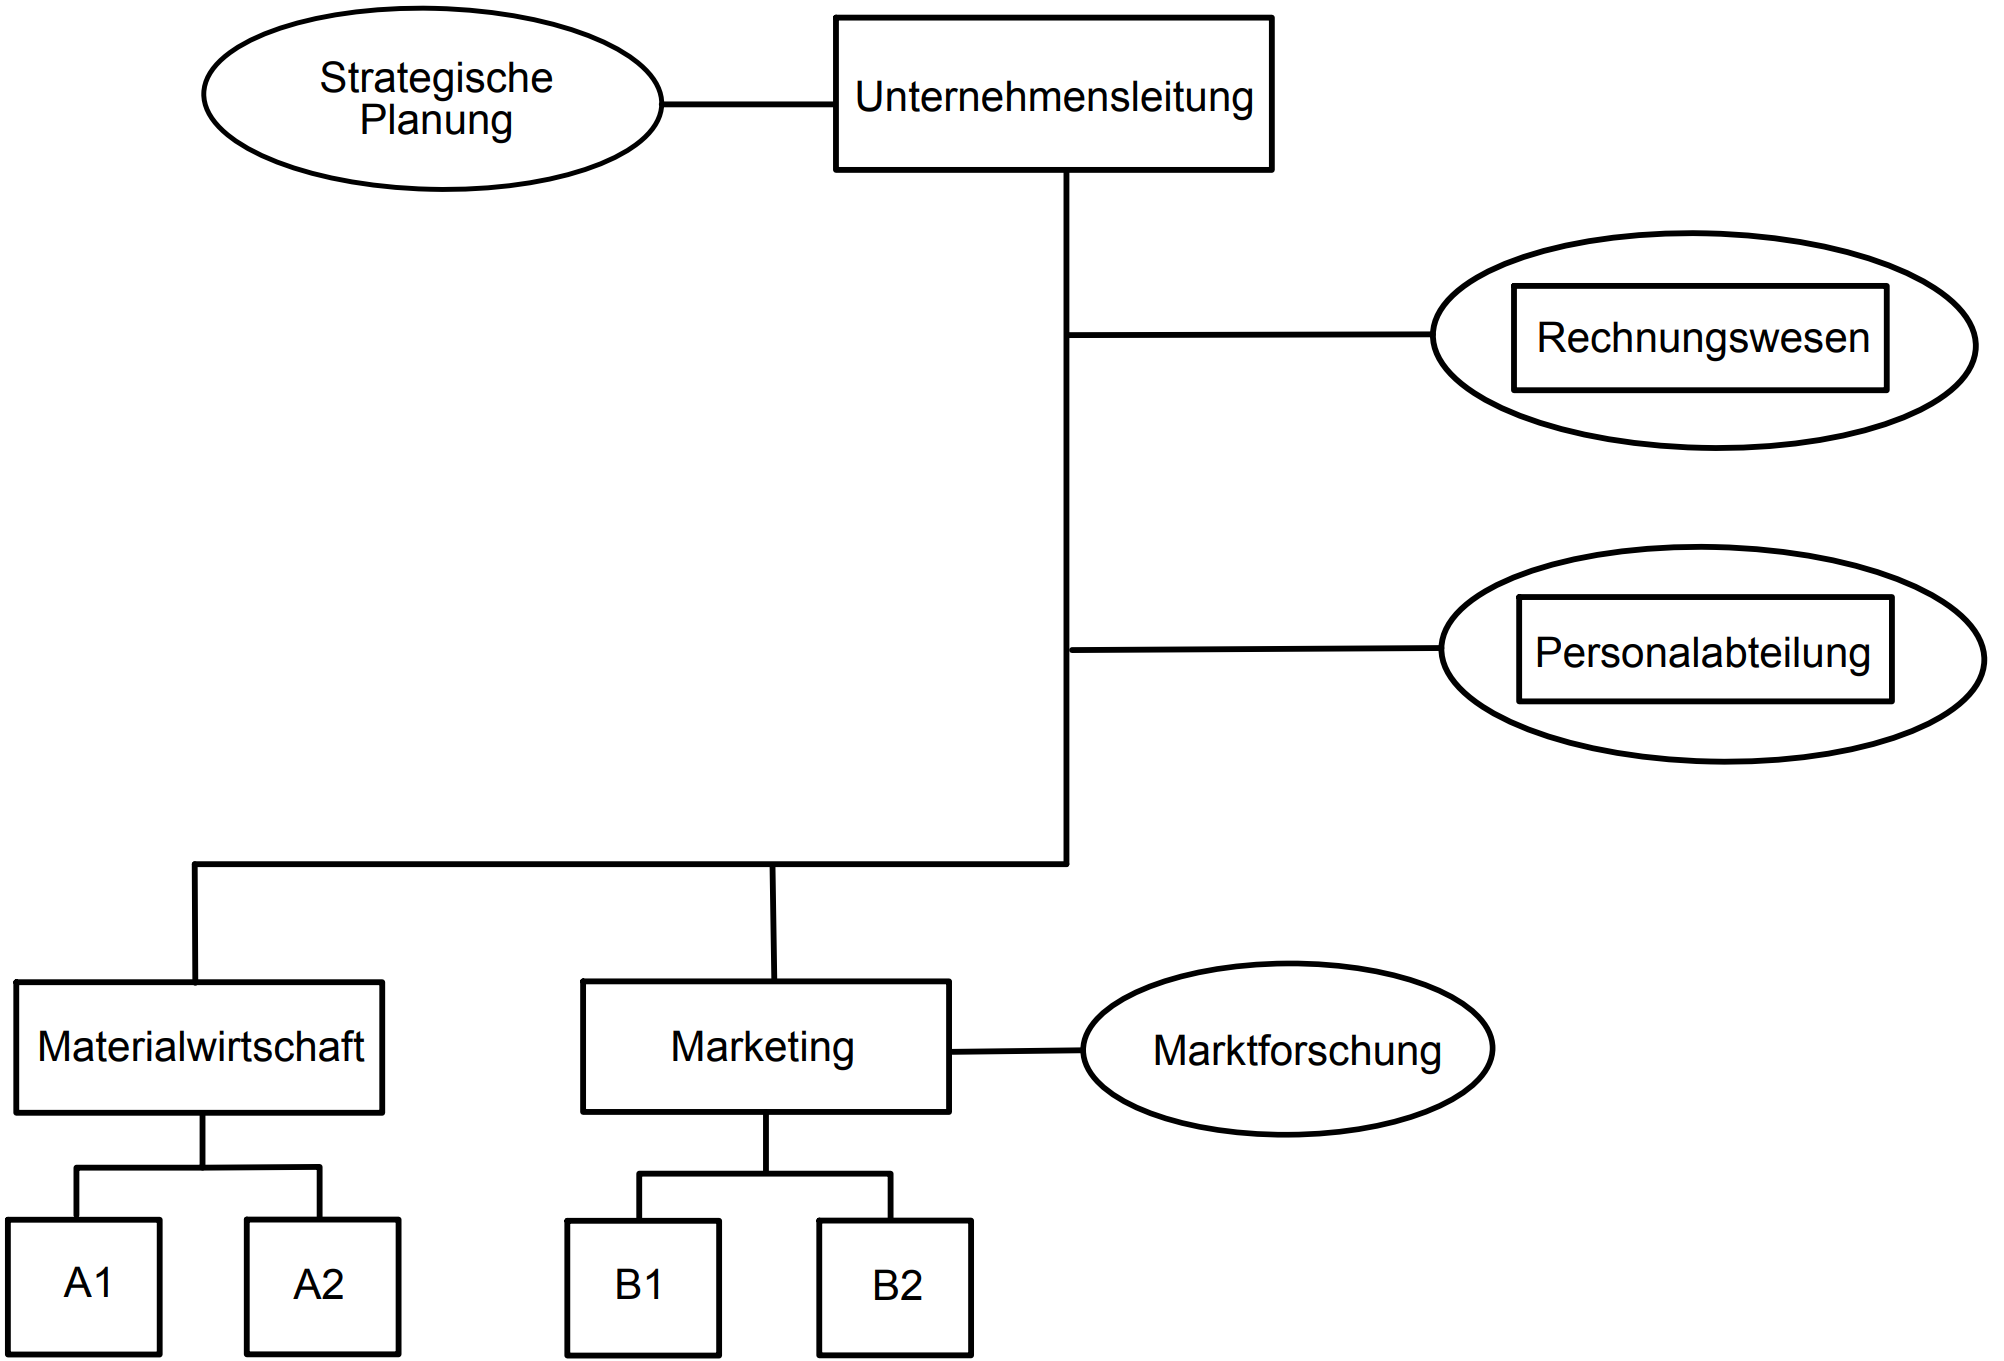
\includegraphics[width = 0.8\textwidth]{Eigene Darstellungen/Stablinienstruktur.PNG}
            \caption{Stabliniensystem (Eigene Darstellung, in Anlehnung an \cite{Woehe2020} S.\,113)} \label{Stablinie}
        \end{figure}

    \subsection{Spartenorganisation} \label{Spartenorganisation}
        In der Spartenorganisation, welche in \fref{Sparte} noch einmal grafisch dargestellt wird, wird das Unternehmen 
        nach Sachgebieten gegliedert. Diese Sachgebiete sind meist Produktgruppen, Absatzgebiete oder Kundengruppen. Die
        Spartenorganisation ist vor allem für Unternehmen geeignet, welche eine sehr heterogene Produktgruppen haben. In 
        dieser Form gibt es jede Abteilung nicht mehr nur einmal, sondern für jede Produktgruppe gibt es alle nötigen 
        Abteilungen noch einmal extra. Das heißt das sowohl die Produktgruppe \emph{A} als auch die Produktgruppe 
        \emph{B} haben eine eigene Marketing Abteilungen. Somit sind diese Abteilungen mehr auf ihr Produkt 
        spezialisiert und können dies unter Umständen besser vermarkten. Dies sorgt auch dafür, das in den höheren 
        Instanzen weniger Aufwand betrieben werden muss, da fast alle notwendigen Entscheidungen in der Sparte selbst 
        getroffen werden. Aufbau dieses Systems ist auch in \fref{Sparte} noch einmal grafisch dargestellt. 
        (Vgl. \cite{Woehe2020} S.\,113-114)

        Diese Organisation kann aber auch zu Problemen führen. Jede Sparte trifft ihre Entscheidungen so, dass diese das 
        für sich beste Ergebnis erzielen, ohne dabei immer Rücksicht auf die anderen Sparten zu nehmen. So kann es zu 
        einem Interessenkonflikt innerhalb des Unternehmens kommen, welcher im schlimmsten Fall zu Umsatzeinbußen führen
        kann. Auch ist diese Organisationsform mit einem hohen verwaltungstechnischen Aufwand verbunden, da die 
        einzelnen Abteilungen mehrfach innerhalb des Unternehmens existieren.

        Durch diese Einteilung können auch weitere Kostennachteile entstehen, wenn zum Beispiel auf ein gemeinsame 
        Produktion verzichtet wird. Auch wenn zum Beispiel in allen Produktgruppen ein bestimmtes Bauteil verwendet 
        wird, aber nicht alle zusammen dieses Bauteil kaufen, kann nicht von Mengenrabatten profitiert werden, was zu 
        erhöhten Kosten in der Materialbeschaffung führt. (Vgl. \cite{Woehe2020} S.\,115)

        \begin{figure}[ht]
            \centering
            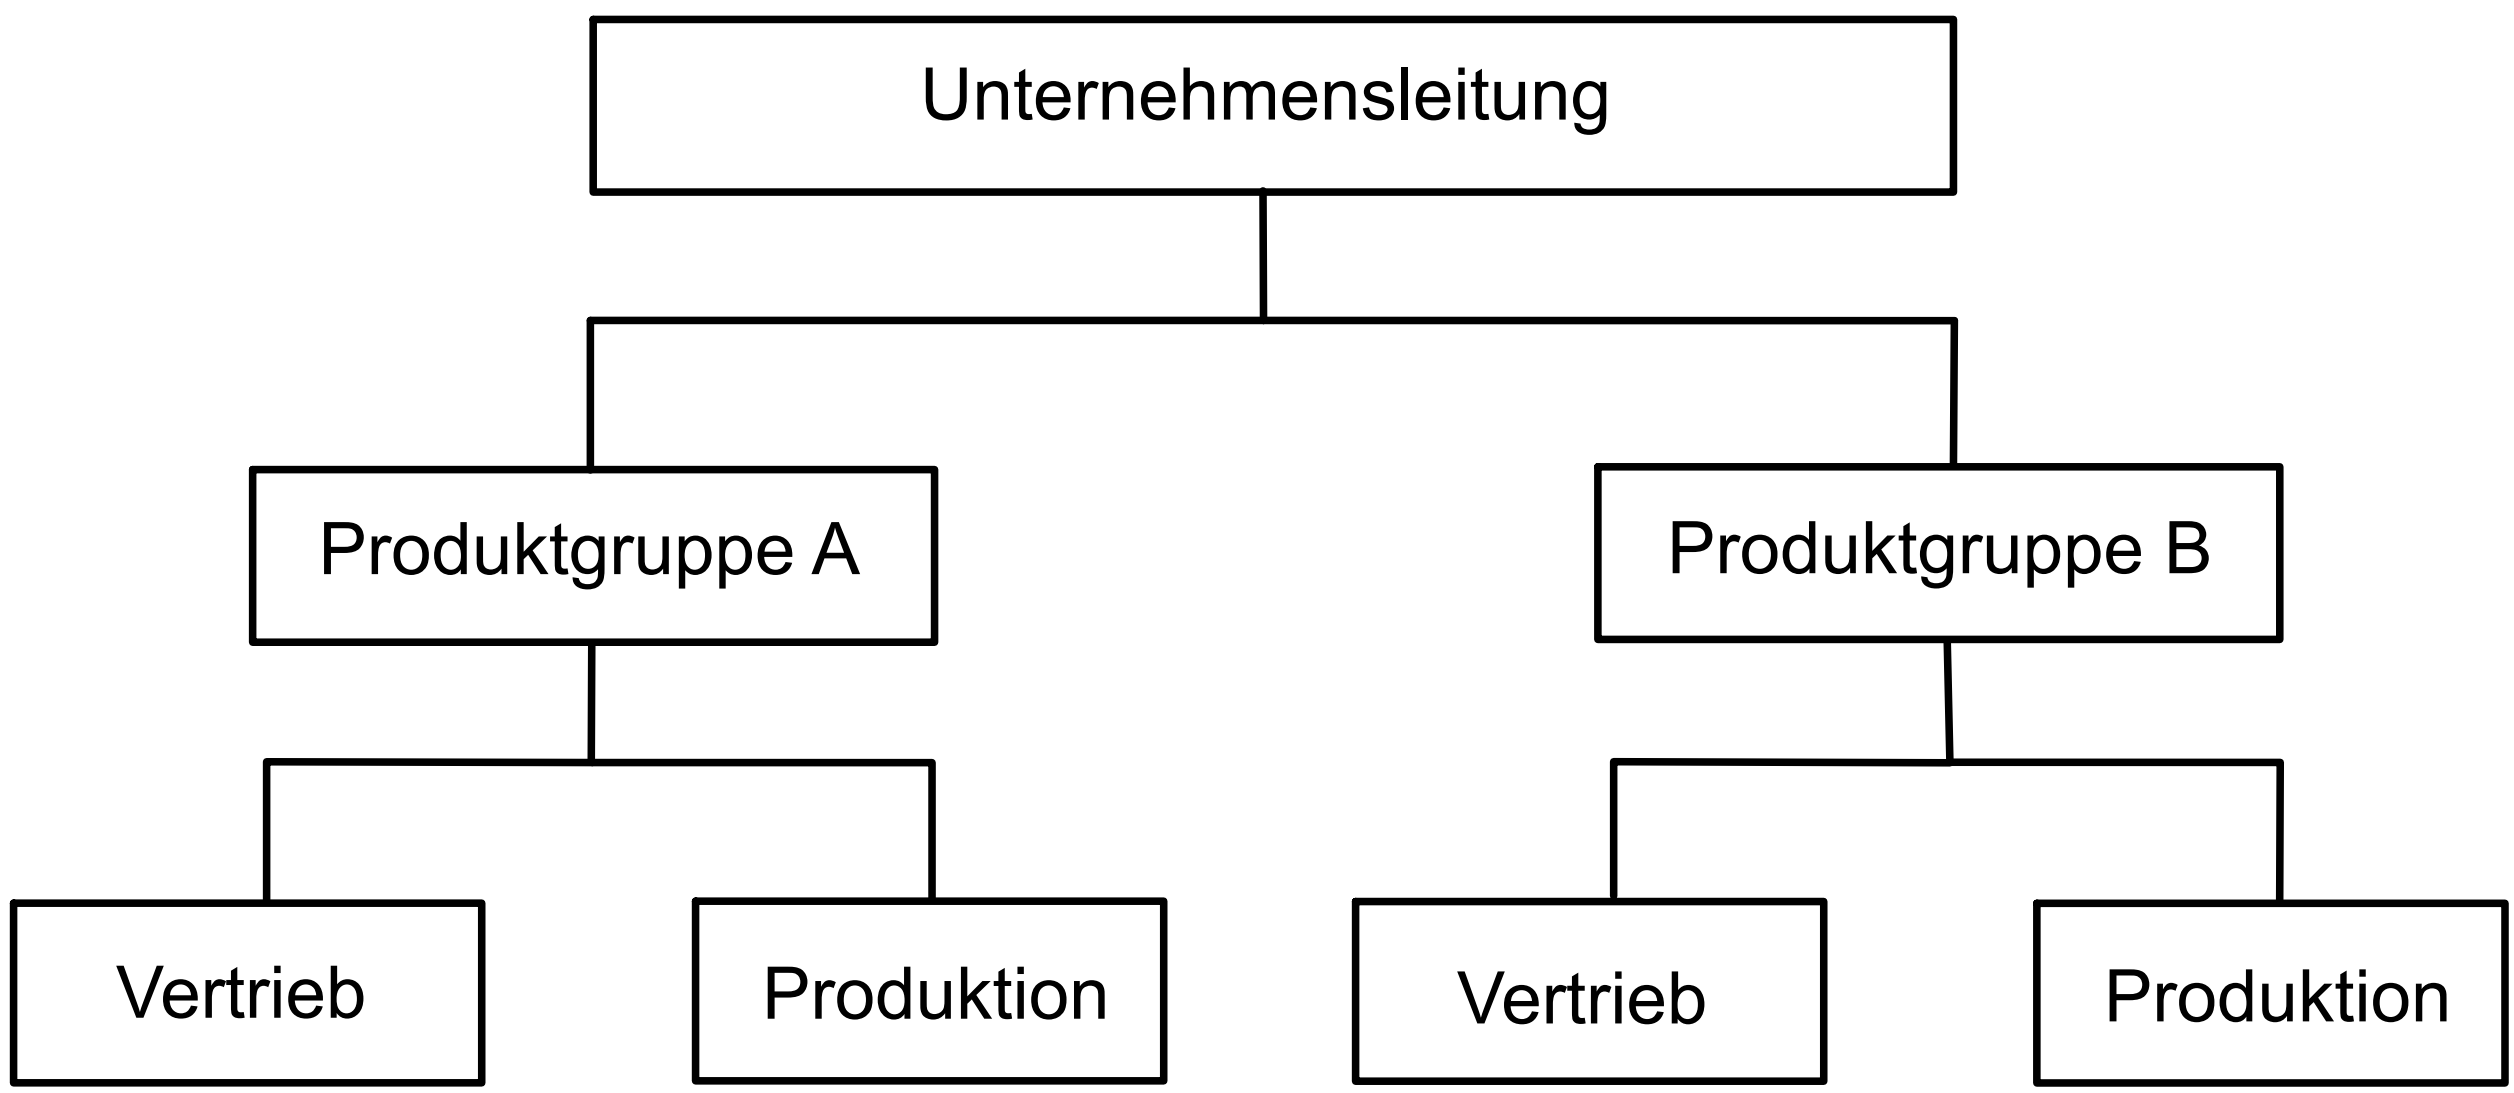
\includegraphics[width = 0.9\textwidth]{Eigene Darstellungen/Spartenorganisation.PNG}
            \caption{Spartenorganisation (Eigene Darstellung, in Anlehnung an \cite{Woehe2020} S.\,114)} \label{Sparte}
        \end{figure}
        

    \subsection{Matrixorganisation} \label{Matrixorganisation}
        Die Matrixorganisation ist ein hybrides System, welches sich vertikal betrachtet auf die die einzelnen 
        Funktionen wie das Marketing oder die Produktion und horizontal auf die Produkte bezieht. Durch diese Verbindung 
        der funktionalen und produktbezogenen Sichtweise können Vorteile in der Koordination gezogen werden. Zum 
        Beispiel durch eine gemeinsame Bestellung der Materialien kann das Unternehmen von Mengenrabatten profitieren 
        und somit einen größeren Umsatz erzielen. (Vgl. \cite{Woehe2020} S.\,115)

        Aber auch hier gibt es Nachteile. An den Knotenpunkten kann es zu organisatorischen Spannungen kommen, wenn es 
        zum Beispiel einen Interessenkonflikt zwischen den Produktverantwortlichen und den Funktionsträgern gibt.
        Ein Beispiel dazu: Der Produktmanager \emph{B} möchte zur Befriedigung individueller Kundenwünsche starke 
        Produktdifferenzierung bei kleinen Stückzahlen, während aber der Projektleiter gar keine Differenzierung möchte
        um die Kosten zu minimieren. (Vgl. \cite{Woehe2020} S.\,115)

        Die Konflikte können auf zwei verschiedene Weisen gelöst werden. Die erste wäre eine Einzelfallentscheidung. 
        Hierbei wird eine Kosten-Nutzen-Analyse durchgeführt, wonach dann entschieden wird, wie die finale Umsetzung 
        erfolgen soll. Die zweite Möglichkeit wäre eine generelle Regelung für häufig auftretende Fälle. Der
        Produktmanager kümmert sich darum, was wann am Markt verfügbar sein soll. Wie die Leistungserstellung allerdings
        abläuft, liegt in der Hand des Funktionsmanagers. Auch das disziplinarische Weisungsrecht über die Mitarbeiter
        liegt beim Funktionsmanager. (Vgl. \cite{Woehe2020} S.\,116)

        \begin{figure}[ht]
            \centering
            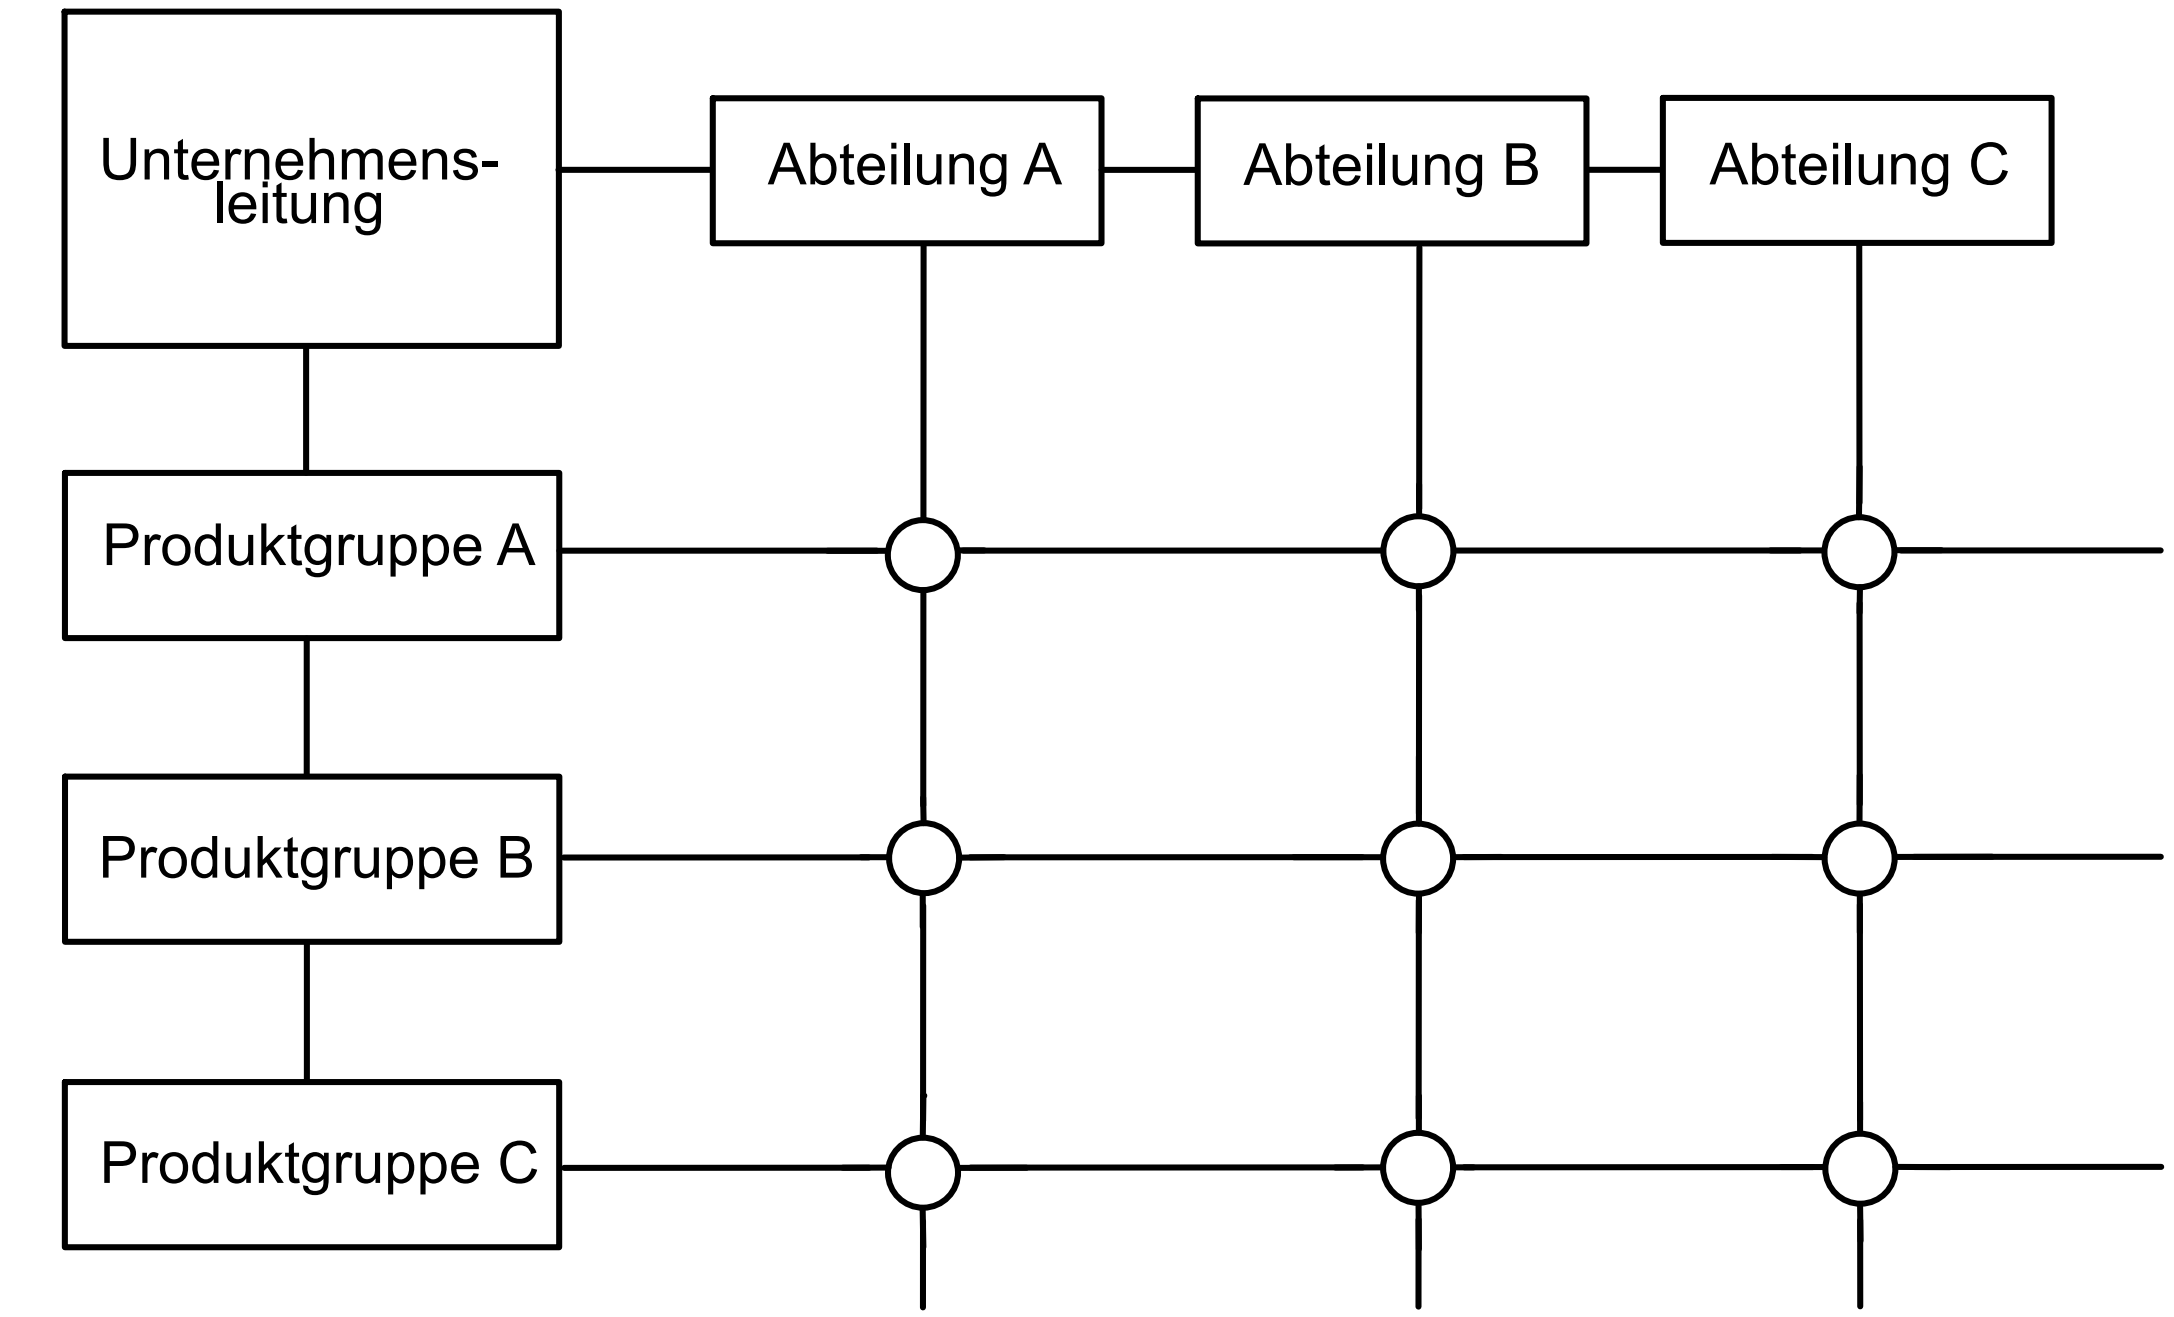
\includegraphics[width = 0.8\textwidth]{Eigene Darstellungen/Matrixstruktur.PNG}
            \caption{Matrixorganisation (Eigene Darstellung, in Anlehnung an \cite{Woehe2020} S.\,115)} \label{Matrix}
        \end{figure}

    \subsection{Organisationsformen bei AMCON} \label{Oformen AMCON}
        Bei AMCON wird als Grundlegende Organisationsform das Einliniensystem (\ref{Einliniensystem}) verwendet. An 
        oberster Stelle steht hier bei die Geschäftsführung, welche sich bei AMCON auf zwei Personen aufteilt. An der
        Geschäftsführung gibt es auch noch 3 Stabstellen. Dazu gehört als erstes die Ausbildung, welche bei uns von 
        einem der Geschäftsführer und einer weiteren Person verwaltet wird. Die beiden anderen Stabstellen sind einmal
        die Unternehmensentwicklung und das strategische Produktmanagement. Unter der Geschäftsführung sind nun direkt 
        alle Abteilungen des Unternehmens untergeordnet. Bei diesen Abteilungen handelt es sich um die Interne IT, die 
        Entwicklung, die Projekte, der Vertrieb und die Verwaltung. Der Bereich der Entwicklung ist der komplexeste 
        Bereich, weshalb ich auf diesen noch etwas näher eingehen werde.

        \begin{figure}[ht]
            \centering
            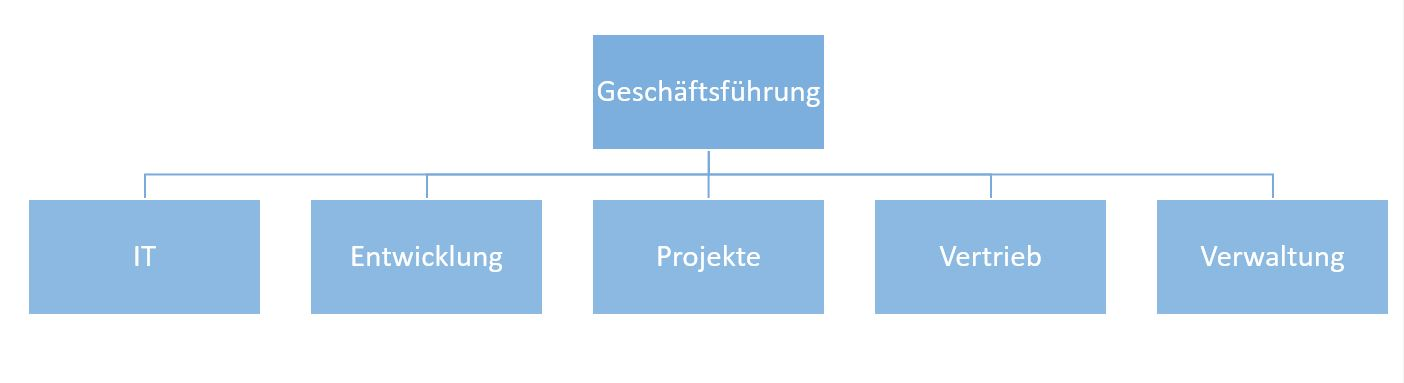
\includegraphics[width = 1\textwidth]{Eigene Darstellungen/OrganigrammEinfach.JPG}
            \caption{Grundlegende Struktur bei AMCON (Interne Dokumentation, Eigene Darstellung)}
        \end{figure}

        An der Abteilung der Entwicklung gibt zwei sogenannte Stabstellen. Das ist einmal der Bereich der Konzeption und
        Architektur und als zweites die Stabstelle der SCRUM Master. Die Abteilung der Entwicklung teilt sich nun, wie
        es in \fref{Entwicklung} zu sehen ist, auf drei weitere Bereiche auf: Entwicklung 1, Entwicklung 2 und das 
        Produktmanagement. Diese drei Bereiche haben alle jeweils einen Abteilungsleiter. Die weitere Gliederung dieses
        Bereichs erfolgt mit der Teamstruktur. Im Bereich \emph{Entwicklung 1} finden wir die Teams Android, Boardunit, 
        PKV, Tarif, Transdev Jobticket und das Team Web. In Bereich \emph{Entwicklung 2} sind die Teams Abo, Hardware, 
        Hintergrundsystem, Kasse und das Team Verkaufsdaten \& Statistik. Im Bereich des Produktmanagements finden sich 
        die Produktmanager, der Support und die Dokumentation wieder.

        \begin{figure}[ht]
            \centering
            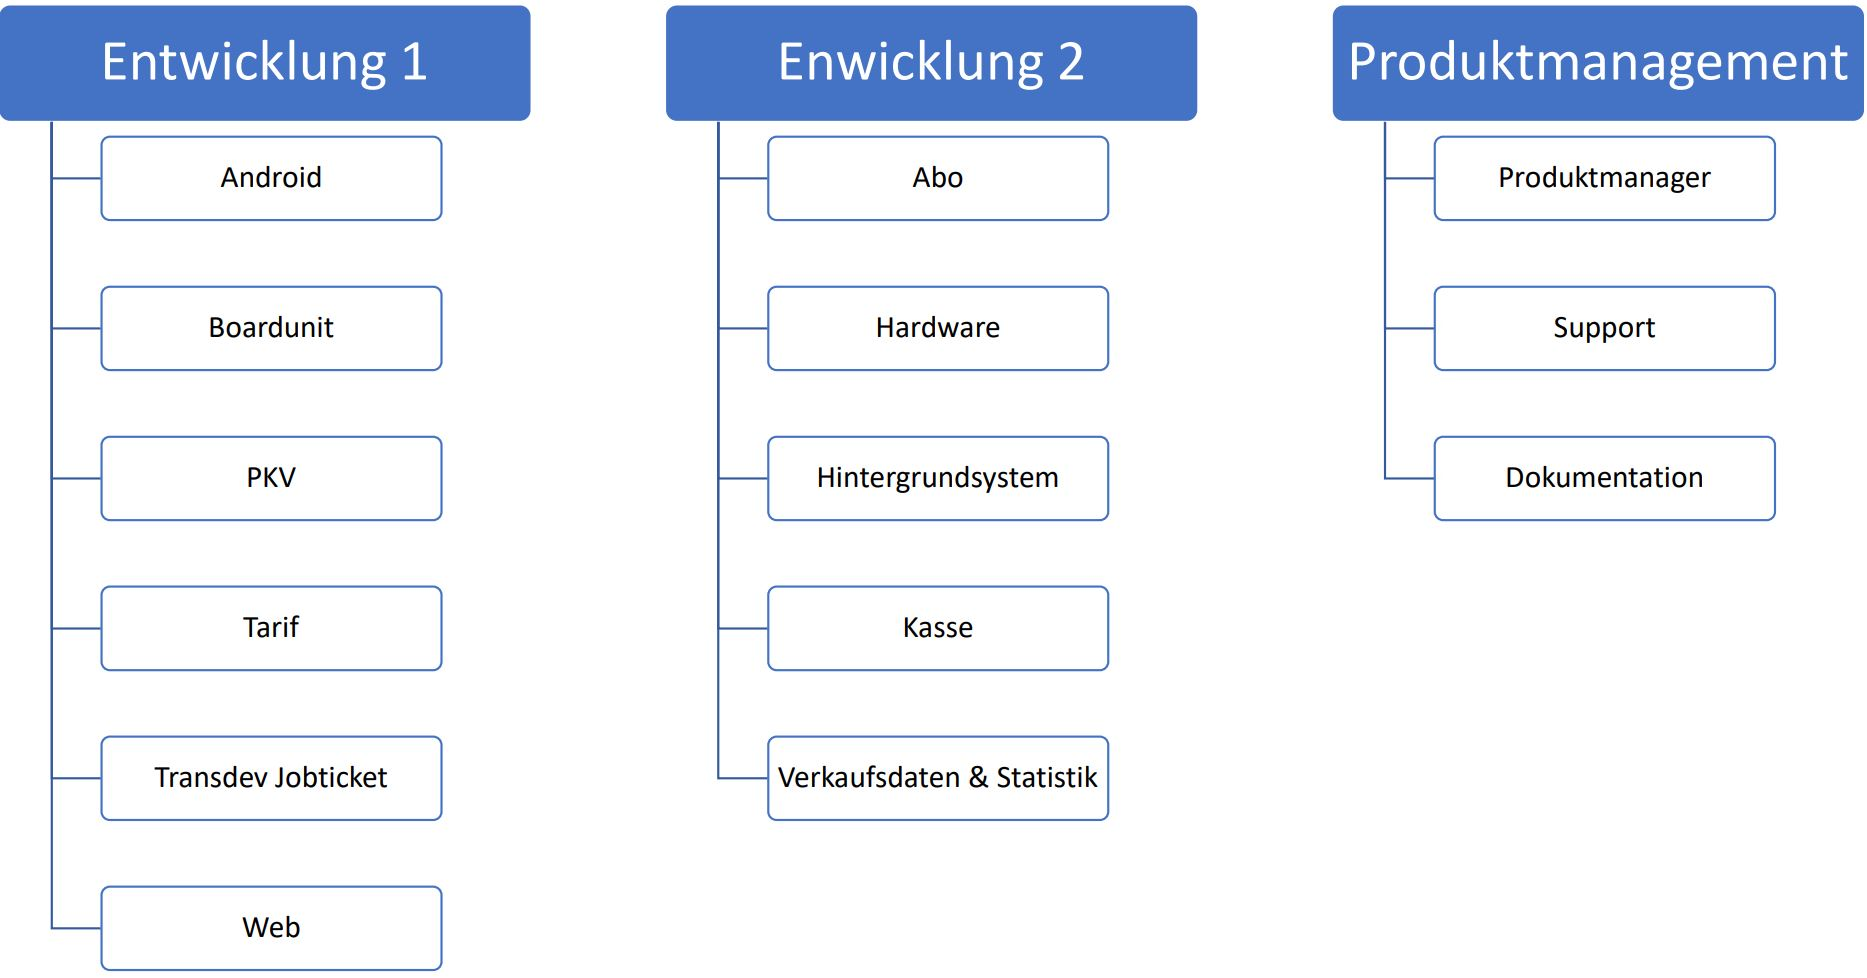
\includegraphics[width = 1\textwidth]{Eigene Darstellungen/Entwicklung.JPG}
            \caption{Organisation der Entwicklungsteams (Quelle: interne Dokumentation, eigene Darstellung)} 
            \label{Entwicklung}
        \end{figure}

        Nach der Dokumentation wird bei AMCON das einfachste der Modelle, das Einliniensystem angewendet. Allerdings
        bilden sich in der Praxis zum Teil auch Mischformen. Durch das Prinzip der \emph{offenen Tür} gilt bei AMCON,
        das jeder Mitarbeiter zu jeder Zeit auf jeden zu gehen kann. Dies schließt auch die Geschäftsführung mit ein.
        Dadurch kommt es in der Praxis also auch häufiger zum Einsatz des Mehrliniensystems, was durch die enge 
        Zusammenarbeit der Entwicklungsteams nicht zu verhindern ist. Würde hier in der Praxis strikt das 
        Einliniensystem angewendet werden, würde dies zu langen und umständlichen Kommunikationswegen führen, welche zu
        einer ineffizienteren Arbeit führen würden.

\section{Führungskonzepte} \label{Konzepte}
    In diesem Kapitel werden die vier verschieden Führungskonzepte Management by Objectives, Exception, Delegation und
    System vorgestellt. Zusätzlich möchte jeweils die Vor- und Nachteile der Konzepte ansprechen und im Anschluss zeigen
    ob und wie diese Konzepte bei AMCON zum Einsatz kommen.
    
    \subsection{Management by Objectives} \label{Objectives}
        Im Management by Objectives wird ein Oberziel formuliert. Dieses Oberziel wird von der Führungsebene zusammen 
        mit den Mitarbeitern in kleinere Teilziele aufgeteilt welche dann von den Mitarbeitern umgesetzt werden. Wie 
        diese Ziele aber erreicht werden, entscheiden die Mitarbeiter selbst. Das bedeutet, dass die Mitarbeiter in 
        diesem Konzept eine größere Verantwortung übernehmen. (Vgl. \cite{Woehe2020} S.\,120)

        Dieses Konzept zielt darauf ab die Mitarbeiter mehr in Entscheidungsprozesse miteinzubeziehen und ihnen mehr 
        Raum für Entscheidungen zu lassen. Dies führt vor allem dazu, das die Motivation der Mitarbeiter gestärkt wird,
        was zu einem höheren Umsatz für das Unternehmen führen kann. (Vgl. \cite{Woehe2020} S.\,120)

        Durch einen Interessenkonflikt zwischen Mitarbeitern und Führungsebene kann es zu Problemen kommen. Das Problem
        ist das die Mitarbeiter durch die Entscheidungsfreiheit auch selbst planen wie lang die Umsetzung dauert. 
        Dadurch kann es dazu kommen, das es Konflikte zwischen Mitarbeitern und Führungsebene kommt, da die Führung 
        nicht mit der Planung der Mitarbeiter einverstanden ist. (Vgl. \cite{Woehe2020} S.\,120)

    \subsection{Management by Exception} \label{Exception}
        Management by Exception funktioniert so, dass der Mitarbeiter seine Aufgaben selbstständig erledigt und die 
        Führungskraft unter \as Normalbedingungen\adl nicht eingreift. Dies passiert nur, wenn das Arbeitsergebnis des
        Mitarbeiters negativ abweicht und in \as kritischen Situationen\adl, also in Ausnahmefällen. 
        (Vgl. \cite{Woehe2020} S.\,119)

        Um dieses System umzusetzen müssen aber einige Fragen im Vorfeld geklärt werden. Dazu gehört zum Beispiel, wie 
        zwischen einem \emph{Normalfall} und einem \emph{Ausnahmefall} unterschieden wird. Auch sollte genau geklärt
        sein, ob es Toleranzbereiche für Abweichung von der Norm gibt. (Vgl. \cite{Woehe2020} S.\,119)

        Dadurch das die Mitarbeiter eher selbstständig arbeiten und weniger Weisung benötigen, wird der Führungsebene
        Arbeit abgenommen. Ein weiterer Vorteil dieses Stils ist die einfache Erkennung von kritischen Situationen, da 
        es schnell auffällt, wenn etwas von der Norm abweicht. Nachteile dieses Konzeptes ist, dass es 
        vergangenheitsorientiert ist. Es werden nur \emph{Soll} und \emph{Ist} mit Werten aus der Vergangenheit 
        verglichen, was dazu führen kann, das sich das Unternehmen nur langsam weiter entwickelt. Ein weiterer Nachteil
        ist die fehlende Motivation der Mitarbeiter. In diesem Konzept bekommen die Mitarbeiter kein Lob oder 
        Anerkennung wenn diese etwas gut gemacht haben. Diese werden nur auf ihre Fehler hingewiesen, was auf Dauer zu
        verringerter Motivation und Arbeitsleitung führen kann. Auch kann dies Auswirkung auf das Allgemeine Arbeitsklima
        im Betrieb haben. (Vgl. \cite{Woehe2020} S.\,\,119)

    \subsection{Management by Delegation} \label{Delegation}
        Bei diesem Führungskonzept werden delegierbare Aufgaben von der Führungsebene an die Mitarbeiter abgegeben. Das
        bedeutet das der Mitarbeiter in diesen Aufgaben Verantwortung über die Umsetzung hat. Das Ziel dieses Systems
        ist es, die Führungsebene durch Abgabe von Routineaufgaben zu entlasten. Außerdem soll dies die Motivation der
        Mitarbeiter stärken, da diese mehr Verantwortung über ihre delegierten Bereiche erhalten. Die Führungskräfte 
        beschränken sich auf eine Erfolgskontrolle. Das heißt das diese einfach nur schauen, ob die Aufgabe richtig 
        ausgeführt wurden. (Vgl. \cite{Woehe2020} S.\,119)

        Die Stärkung der Mitarbeitermotivation klappt mit diesem Konzept allerdings nur bedingt. In den meisten fällen
        werden hauptsächlich die \as lästigen\adl Aufgaben an die Mitarbeiter abgegeben, was sogar eher einen 
        gegenteiligen Effekt haben kann. So kann es auch dazu kommen, das die Aufgaben auf Dauer nicht mehr so gut 
        ausgeführt werden. (Vgl. \cite{Woehe2020} S.\,119)

    \subsection{Management by System} \label{System}
        Mit Management by System wird die Führung des Betriebs vor allem durch ein computergestütztes Planungs-,
        Kontroll- und Informationssystem gehandhabt. Mit diesem Führungskonzept wird das Ziel der Totalplanung verfolgt.
        Das bedeutet, das jeder einzelne Arbeitsschritt mit einem computergestütztem System durchgeplant ist.
        (Vgl.\cite{Woehe2020} S.\,120)

        Allerdings bleibt bei diesem Führungskonzept eine offene Frage, ob ein Computersystem menschliche Erfahrung und 
        Intuition ersetzen können. Hier kann es Situation geben, in welchen das System die richtige Entscheidung treffen
        kann. Allerdings gibt es auch Situationen, welche von einem Menschen beurteilt werden müssen. Darunter würde zum
        Beispiel das generelle Personalwesen fallen. Eine Computersystem kann hier nur nach Fakten beurteilen. Aber ein
        Mensch ist hier in der Lage besser einen anderen Menschen zu beurteilen, ob dieser zum Beispiel in das Team 
        passt oder nicht. (Vgl. \cite{Woehe2020} S.\,120)

        Der Vorteil dieses Systems sind die gesamte Verbesserung der Planungs-, Kontroll- und Informationsstruktur.
        Durch ein computergestütztes System können Abweichungen vom \as Normalzustand\adl schneller erkannt werden und
        es können schneller Maßnahmen zur Behebung eines Problems eingeleitet werden. (Vgl. \cite{Woehe2020} S.\,120)

        Nachteile sind allerdings, das dieses System keine Motivations für die Mitarbeitet mit sich bringt, sondern eher
        das Gefühl der Überwachung. Auch wird den Mitarbeitern hier nicht viel Verantwortung übertragen, da durch das 
        System der gesamte Arbeitsprozess durchgeplant ist. (Vgl. \cite{Woehe2020} S.\,120)

        Dies alles führt dazu, dass durch das Informationssystem allenfalls Routineprozesse durchgeführt werden können,
        bei welchen keine Menschliche Einschätzung der Situation von Nöten ist. (Vgl. \cite{Woehe2020} S.\,120)

    \subsection{Führungskonzepte bei AMCON} \label{Konzepte AMCON}
        Bei AMCON wird das Projektmanagement SCRUM genutzt, auf welches im Kapitel \ref{SCRUM} der Ausarbeitung noch 
        näher eingegangen wird. Mit diesem Management entsteht ein Mischform aus \emph{Management by Exception} 
        (\ref{Exception}) und \emph{Management by Objectives} (\ref{Objectives}). Im SCRUM-Prozess gibt es sogenannte
        Sprints welche normalerweise circa einen Monat dauern. Zu beginn des Sprints wird dieser geplant, wobei alle 
        beteiligten Entwickler die einzelne Aufgaben besprechen und planen, wie Aufwendig diese sind. Nach der Planung
        beginnt der Entwicklungsprozess. Während dieser Zeit arbeiten die Entwickler selbstständig an den vorher 
        geplanten Aufgaben. Nur bei Fragen oder Problemen, welche der Entwickler selbst nicht lösen kann oder hierzu 
        nicht befugt ist eine Entscheidung zu treffen, schreitet der Teamleiter ein. Nachdem der Entwickler eine Aufgabe 
        abgeschlossen hat nimmt dieser sich selbstständig die nächste Aufgabe aus dem Sprint. Die Aufgaben mit höchsten
        Priorität werden als erstes bearbeitet.

        Während der Einarbeitungsphase ist die Freiheit noch nicht ganz so groß. Hier kommt eher \emph{Management by 
        Delegation} (\ref{Delegation}) zum Einsatz. Hier kann die Azubis bzw. mich selbst als Beispiel nehmen. Als ich
        im August meine Ausbildung begonnen habe, habe ich Aufgaben zugeteilt bekommen, mit welchen ich zuerst die 
        Grundlagen der Programmierung erlernt habe. Danach habe ich Aufgaben bekommen, mit welchen ich mich in das 
        Produkt meines Teams einarbeiten konnte. Mittlerweile ist bei mir eine Mischform aus \emph{Management by 
        Delegation} und dem normalen Prozess entstanden. In den meisten Fällen nehme ich mir meine Aufgaben selbst aus 
        dem Sprint. Es kommt aber immer noch vor, das ich auch Aufgaben von meinem Teamleiter zugewiesen bekomme.

\section{Team Verkaufsdaten \& Statistik} \label{TeamVS}
    Seit dem Beginn meiner Ausbildung arbeite ich im \emph{Team Verkaufsdaten \& Statistik}(Team VS). Unser Team arbeitet wie die
    meisten Teams bei AMCON im HGS. Dabei übernehmen wir Teilbereiche wie die Nebenbuchhaltung, die Verkäuferkonten und 
    die Schichtenverwaltung. Dies sind drei der Module welche es bei uns im HGS gibt. In den nachfolgende Kapiteln werde
    ich einmal unser Projektmanagement SCRUM vorstellen. Im zweiten Unterpunkt werde ich dann vorstellen wie wir bei uns
    im Team VS zur Zeit arbeiten und im folgenden dann auf die Vor- und Nachteile dieser Arbeitsweise eingehen. Zum 
    Abschluss dieses Kapitels werde ich mögliche Verbesserungsvorschläge geben um den Prozess effizienter zu gestalten.

    \subsection{SCRUM Projektmanagement} \label{SCRUM}
        Bei AMCON kommt das Projektmanagement SCRUM zum Einsatz. Dabei handelt es sich um eine agile Projektmanagement
        Methode, mit welcher schnell und einfach auf Veränderungen im Projekt reagiert werden kann.

        Bei SCRUM gibt es die sogenannten \emph{Sprints}. Jeder Sprint dauert circa einen Monat. Vor beginn des Sprints
        wird dieser geplant. Zur Planung gehört das schreiben der sogenannten \emph{User Storys}. Diese werden bei uns
        in Form von \emph{Tickets} geschrieben. Diese Tickets werden dann von den Projektleitern, 
        Produktverantwortlichen und Teamleitern priorisiert. Das heißt es wird geschaut, welche dieser Aufgabe als 
        erstes bearbeitet werden müssen. Danach werden diese Tickets an die Entwicklungsteams gegeben welche sich dann
        die Tickets anschauen und diese schätzen. Beim schätzen werden den Tickets \emph{Storypoints} zugewiesen. Je
        mehr Punkte ein Ticket bekommt, desto aufwendiger ist es. Nachdem alle Ticket geschätzt sind und der Sprint
        vollständig geplant ist, beginnt die Entwicklungsphase. In dieser Zeit arbeiten die Entwickler an der Umsetzung
        der eingeplanten Tickets. Jeden Tag gibt es dazu noch die \emph{Daily's}. Dies sind Termine in denen sich alle 
        Mitglieder eines Teams einmal am Tag zusammen finden und besprechen, was diese seit dem letzten Daily gemacht 
        haben. Diese Termine können auch gut dafür genutzt werden um Fragen zu klären und einen aktuellen Stand der 
        anderen Teammitglieder zu bekommen. Am Ende des Sprints gibt es einen \emph{Review Termin}. In diesem Termin 
        stellen die Entwickler ihre abgeschlossenen Tickets den Projektleitern und Produktverantwortlichen vor. Während
        der RC-Woche (Release Candidate) werden alle implementierten Funktionen noch einmal getestet, um 
        sicherzustellen, dass keine Fehler entstanden sind. In der Retrospektive bespricht das Entwicklungsteam dann 
        noch einmal was im letzten Sprint gut und was schlecht gelaufen ist. Auch werden Vorschläge gemacht, wie Dinge 
        besser umgesetzt werden können. Durch diese regelmäßigen Besprechungen, sind wir als Entwicklungsteam in der 
        Lage uns stetig weiter zu entwickeln und Probleme zu beheben, welche uns während der Entwicklungsphase 
        aufgefallen sind. Ein detaillierter Ablauf unseres SCRUM-Prozesses ist auch noch einmal in \fref{SCRUMProzess}
        zu sehen.

        \begin{figure}
            \centering
            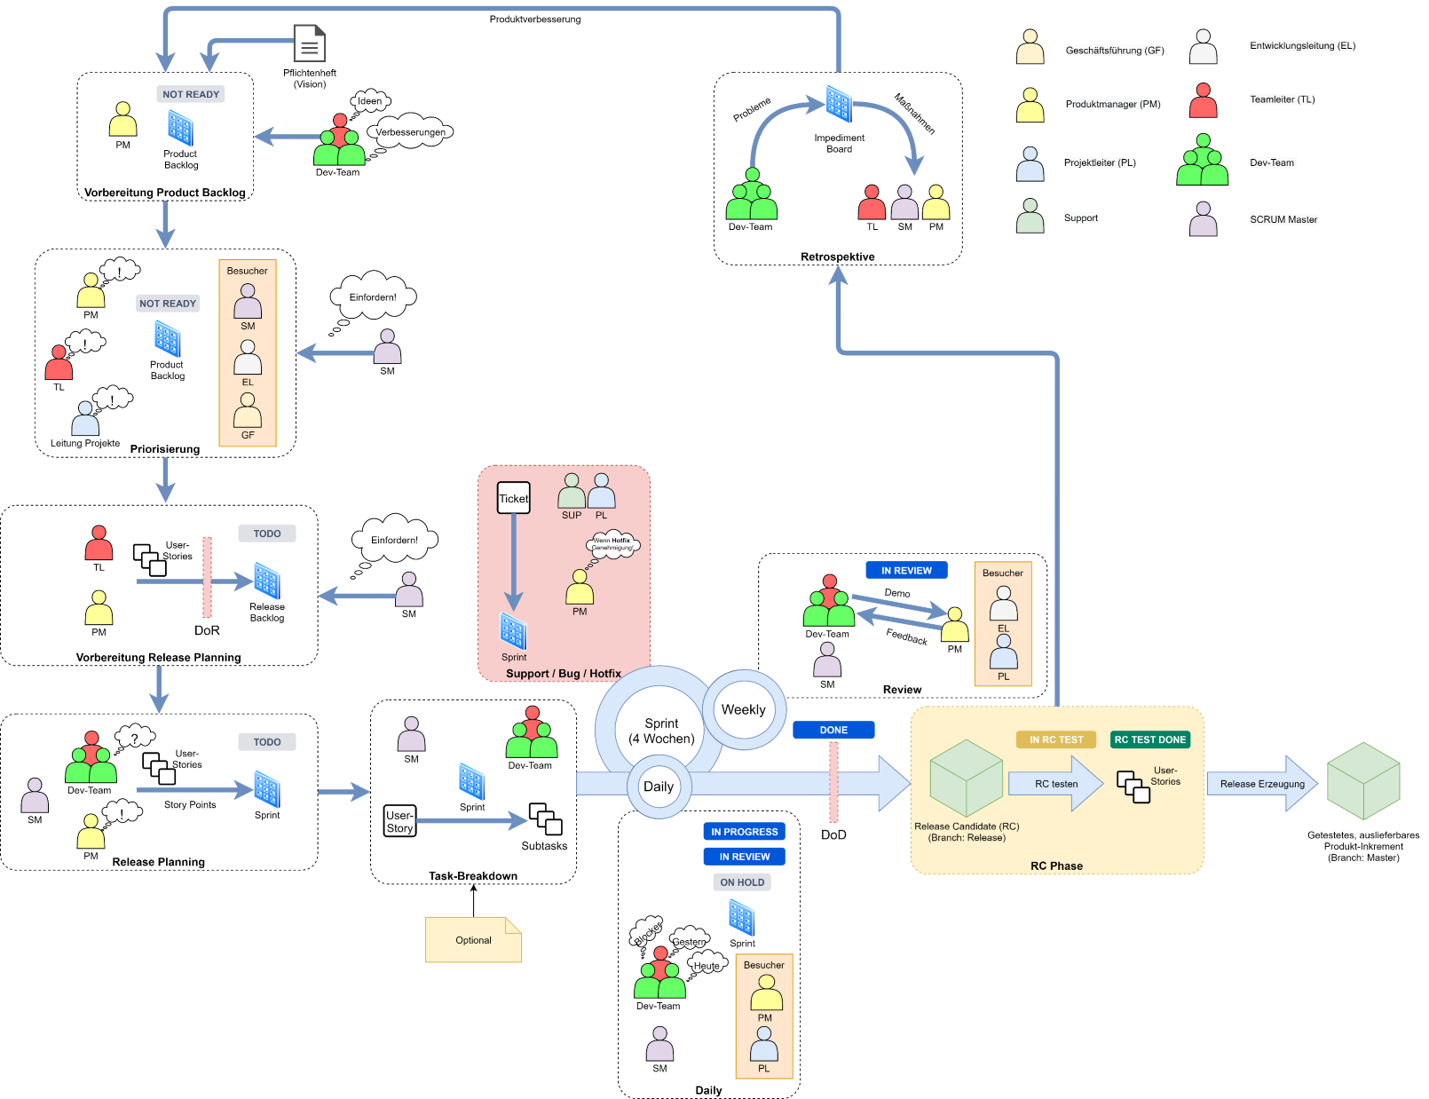
\includegraphics[width = 0.8\textwidth]{Eigene Darstellungen/SCRUM.png}

            \caption{SCRUM-Prozess bei AMCON (Quelle: Interne Dokumentation)} \label{SCRUMProzess}
        \end{figure}

    \subsection{Wie arbeiten wir in unserem Team?} \label{Aktuell Team VS}
        Das Team VS besteht aus einem Teamleiter, einem Entwickler und zwei dualen Studenten. Zur Zeit haben wir auch
        noch einen Entwickler aus dem Team Hintergrundsystem zur Unterstützung bekommen. Indirekt gehört auch noch
        ein Produktmanager zum Team dazu. Dieser hat aber mit der eigentlichen Entwicklung nichts zu tun.

        Nach dem Start eines neuen Projektes erstellen die Projektleiter zusammen mit dem Kunden das Pflichtenheft, in 
        welchem festgehalten ist, welche Anforderungen das fertige Produkt erfüllen muss. Nach Festlegung der 
        Anforderungen werden die Anforderungen in Tickets aufgeteilt, welche dann im späteren Verlauf von den 
        Entwicklungsteams selbst im Aufwand eingeschätzt werden. 

        Angekommen im eigentlichen Entwicklungsprozess greift hier nun das \emph{Management by Exception} 
        (\ref{Exception}). Das heißt das vom Teamleiter oder von den Produktverantwortlichen nur noch in Ausnahmefällen
        eingegriffen wird. Es kann aber immer mal vorkommen, das erst während der eigentlichen Entwicklung bestimmte 
        Randfälle auffallen, welche dann noch einmal separat mit einem anderen Team oder den Produktverantwortlichen
        abgesprochen werden muss. Dies führt zu viel interner Kommunikation, welche häufig viel Zeit in Anspruch nehmen
        kann.
        
        Innerhalb des Teams steht der Teamleiter immer für Fragen zur Verfügung, da dieser einerseits das Produkt und 
        Technik aber auch die Anforderungen kennt. Der Teamleiter dient als Führungsinstanz für sein Team, ist aber auch
        aktiv mit am Entwicklungsprozess beteiligt.

    \subsection{Vor- und Nachteile dieser Arbeitsweise} \label{VorNachteile}
        Durch die Teamstruktur welche bei AMCON umgesetzt wird, entstehen aber auch für Probleme. Bei AMCON müssen die 
        Teams sehr viel miteinander kommunizieren und sich gegenseitig abstimmen, wie genau eine bestimmte Anforderung 
        umgesetzt wird. Der Grund hierfür ist die Aufteilung unsere Softwarelösung auf die verschiedenen Teams. Hierzu 
        einmal ein Beispiel. Wenn zum Beispiel in unserem Team ein neuer Export umgesetzt werden soll oder ein bereits
        bestehender erweiter werden soll und hierfür Daten benötigt werden, welche zum Beispiel aus dem Team der 
        Boardunit kommen, müssen wir uns vorher abstimmen, wie diese Daten aussehen sollen, damit wir in unserem Team 
        damit auch gut arbeiten können. 
        
        Auch ist es wichtig, das wir uns gut Absprechen beim Thema Software Release. Es darf nicht passieren, dass zum 
        Beispiel in der Boardunit ein neues Feature umgesetzt und an den Kunden geht, welches auf ein anderes Feature im
        HGS aufbaut, das noch nicht implementiert wurde. Wenn das passieren würde, würde es im System des Kunden zu 
        Fehlern kommen, welche eine negative Auswirkung auf das Unternehmen und die Beziehung zum Kunden hätten.

        Diese Probleme werden aktuell durch sehr viel Kommunikation zwischen den einzelnen Entwicklungsteams gelöst. 
        Dies führt allerdings dazu, das weniger Zeit für die eigentliche Entwicklung der Software bleibt und mehr für
        die Besprechung der Umsetzung verwendet wird. Auch gibt es durch unterschiedlichen Arten der Kommunikation
        das Problem, das manchmal nicht mehr nachvollzogen werden kann, wo genau was zu einem bestimmten Ticket 
        besprochen wurde. Neben den konventionellen E-Mails, gibt es bei AMCON auch noch ein Tool names \emph{Slack}, 
        welches zur schnellen internen Chat-Kommunikation verwendet wird. Außerdem gibt es die Möglichkeit mit anderen
        Leuten persönlich zu sprechen oder mit diesen zu telefonieren. Unter den Tickets selbst können auch 
        Kommentare geschrieben werden.

        Um das Problem der nicht immer nachvollziehbaren Kommunikation zu lösen gibt es verschiedene Möglichkeiten. Zum
        einen könnte das die Kommunikation auf einen Weg beschränkt werden. Zum Beispiel E-Mails. Allerdings ist es 
        deutlich umständlicher Dinge über E-Mails zu besprechen, wenn viele Personen daran beteiligt sind. Hier für sind 
        Chatrooms besser geeignet. Mein Ansatz um dieses Problem zu lösen wäre aber nicht die gesamte Kommunikation auf 
        nur einen Kommunikationsweg zu beschränken, sondern eine generelle Regel einzuführen, das wenn Dinge zu einem 
        Ticket besprochen werden, dies immer in den Kommentaren unter dem Ticket zu machen bzw. wenn mehr Leute 
        beteiligt sind dies in einem Meeting zu machen und das Besprochene anschließend im bzw. am Ticket festzuhalten.

        Dies würde aber noch nicht wirklich das Ursprüngliche Problem der übermäßigen Kommunikation lösen. Eine 
        Möglichkeit wäre engere Vorgaben zu machen. Das bedeutet, wenn die relativ Flache Hierarchie bei AMCON mehr Zu
        einer \emph{Top-Down Struktur} werden würde, könnte genau vorgegeben werden, wie genau einzelne Dinge umgesetzt
        werden müssen. Allerdings hätte dies wieder den Nachtteil, dass die Entwickler nicht so eigenständig arbeiten 
        könnten. Wenn es hier zu Problemen bei der Umsetzung kommen würde, wäre es schwieriger eine schnelle Lösung
        zu finden, da jede Anpassung noch einmal genau Abgesprochen werden müsste.

        Mein Fazit ist also, dass es nur schwierig umsetzbar ist die benötigte Kommunikation zwischen den einzelnen
        Entwicklungsteams zu verringern, ohne dabei die grundsätzliche Struktur zu verändern, was wiederum zu neuen 
        Problemen führen würde. Allerdings kann der aktuelle Stand dahingehend verbessert werden, das möglicherweise
        allgemeine Regeln zur Besprechung von zum Beispiel Tickets eingeführt werden, um hier ein klare 
        Nachvollziehbarkeit gewährleisten zu können.

\section{Ethisch- und Praktisch-normativ}
    In diesem Abschnitt werde ich einmal auf den Unterschied zwischen der ethisch- und praktisch-normativen 
    Betriebswirtschaftslehre eingehen. Im Anschluss werde ich schauen, ob es sich bei AMCON eher um ein ethisch- oder 
    praktisch-normatives Unternehmen handelt und warum dies der Fall ist.

    \subsection{Definition ethisch- und praktisch-normativ}
        In der Betriebswirtschaftslehre wird zwischen zwei Werturteilen unterschieden: den primären und den sekundären.
        Bei den primären Werturteilen handelt es sich um die Ethisch-normative Betriebswirtschaftslehre. Die beschäftigt
        sich vor allem mit moralischen Wertvorstellungen und legt das Wohlbefinden der Arbeitnehmer in den Vordergrund.
        Was aber nun wirklich moralisch ist und was nicht kann nicht wissenschaftlich belegt werden. Hier hat jeder 
        seine eigene Meinung. Zum Beispiel kann gesagt werden: Die Partizipationsrechte der Arbeitnehmer müssen gestärkt
        werden. Hierbei wird immer moralisch gehandelt. Gewinnmaximierung gilt als unmoralisch.

        Neben der Ethisch-normativen Betriebswirtschaftslehre gibt es auch die praktisch-normative 
        Betriebswirtschaftslehre, die sekundären Werturteile. Hierbei gilt zum Beispiel: Wer Gewinne maximieren will,
        darf das ökonomische Prinzip nicht verletzen und darf auch nicht auf eine Kontrolle der Wirtschaftlichkeit 
        verzichten. In der praktisch-normativen BWL wird nicht unterschieden, ob etwas moralisch oder unmoralisch ist.
        Wenn etwas den Gewinn steigert, ist es umzusetzen. Da hier nicht unterschieden werden muss, ob etwas moralisch 
        ist oder nicht, kann dies auch wissenschaftlich belegt werden. Hier fließt keine persönliche Meinung mit ein.

    \subsection{Ist AMCON ethisch- oder praktisch-normativ?}
        AMCON ist ein Unternehmen, welches viele Aspekte der Ethisch-normativen Betriebswirtschaftslehre erfüllt. Dazu
        gehört zum Beispiel, das bei AMCON die Zufriedenheit der Mitarbeiter und Kunden einen sehr hohen Stellenwert
        hat. (Vgl. \cite{AMC22c}) Dies wird auch genauso umgesetzt: Es gibt häufig Mitarbeiterevents wie die monatliche 
        Mitarbeiterrunde oder auch Events zusammen mit Kunden. Dazu gibt es für die Mitarbeiter Benefits wie zum 
        Beispiel ein reduziertes Mittagessen bei Kooperationspartnern oder kostenlose Getränke. Auch wurde AMCON schon 
        mehrmals mit dem Preis \as Beste Arbeitgeber Niedersachsen Bremen\adl ausgezeichnet. Im Jahr 2020 hat AMCON auch 
        den Preis \as Beste Arbeitgeber ITK\adl bekommen. (Vgl. \cite{AMC22B})

        AMCON erfüllt Aspekte der Ethisch-normativen BWL allerdings ist es nicht in dieser Sparte einzuordnen. Bei AMCON
        steht immer noch die Gewinnmaximierung im Vordergrund. Durch die Erfüllung der Ethisch-normativen Aspekte zielt 
        AMCON darauf ab die Mitarbeiter- und Kundenzufriedenheit zu stärken und diese damit langfristig an sich zu 
        binden, was eine Steigerung des Gewinns mit sich zieht. Somit ist AMCON eindeutig als praktisch-normatives 
        Unternehmen einzuordnen.

\section{Rückblick und Fazit des Projektes}
    Rückblickend hat mir dieses Projekt dahingehend geholfen, die gelernte Theorie des ersten Semesters noch einmal zu 
    wiederholen und alles zu festigen. Die Anwendung auf die Praxis allerdings fiel mir in einigen Teilen recht schwer,
    da ich nicht immer genau sagen konnte, welches Führungskonzept nun genau bei AMCON verwendet wird. In der Praxis 
    kommt es häufiger zu Mischformen der einzelnen Konzepte. Im Fall der Organisationsstruktur bin ich auf das gleiche 
    Problem gestoßen, da ich auch hier nicht genau sagen konnte, welche Struktur nun genau verwendet wird. 

    Dass ich auf diese Probleme gestoßen bin, zeigt, dass es sich bei den Führungskonzepten und Organisationsformen um 
    nichts anderes als Modelle handelt. In der Theorie gilt zum Beispiel beim Einliniensystem, das der Ansprechpartner
    immer die nächst höhere Person in der Hierarchie ist. In der Praxis allerdings wird dies aber weniger umgesetzt,
    da es zu langen und ineffizienten Kommunikationswegen führt.

    Diese Konzepte werden in gewisser Form in den meisten Unternehmen zu finden sein. Bei AMCON aber wurden die Konzepte 
    auf das Unternehmen und die gewünschte Arbeitsweise und die Bedürfnisse des Unternehmens angepasst. Dies ist etwas,
    dass nach meiner Vermutung auch in andere Unternehmen so gemacht wird. Es ist also schwierig die Theorie immer 
    1:1 auf die Praxis zu übertragen, da es hier immer zu Abweichungen kommen wird.